% Modified from Figure 5.5 on Bondy and Murty's Graph Theory with Applications, p.75.
\documentclass[border=2mm,12pt]{standalone}
\usepackage{tikz}

\usetikzlibrary{calc,decorations.pathreplacing}

\begin{document}
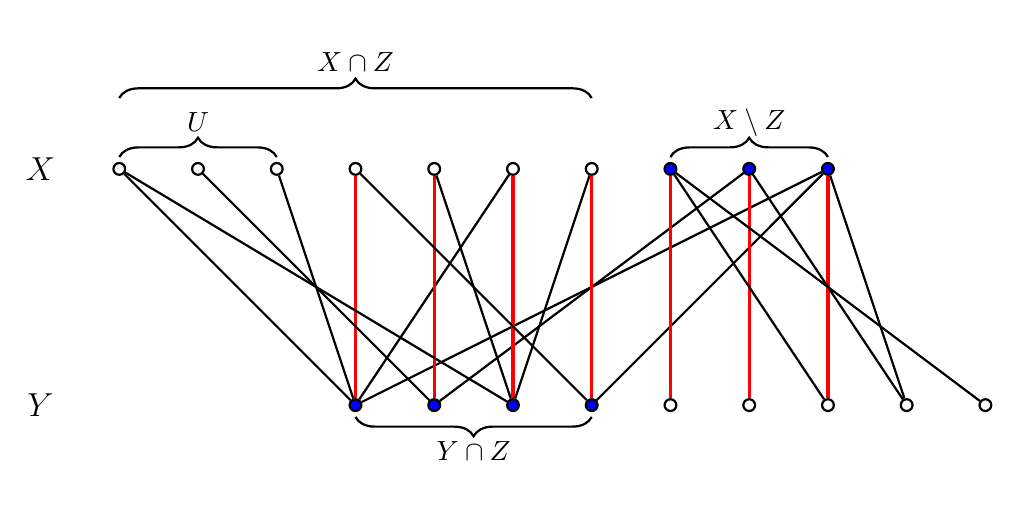
\begin{tikzpicture}[
    yscale=1.5, thick,
    every node/.style={draw, circle, inner sep=-1.5pt},
]

    \foreach \i in {-3,...,3} {
        \node (x\i) at (\i, 2) {};
    }

    \foreach \i in {4,...,6} {
        \node [fill=blue] (x\i) at (\i, 2) {};
    }

    \foreach \i in {0,...,3} {
        \node [fill=blue] (y\i) at (\i, 0) {};
    }

    \foreach \i in {4,...,8} {
        \node (y\i) at (\i, 0) {};
    }

    \draw (x-3) -- (y0);
    \draw (x-1) -- (y0);
    \draw (x0)  -- (y0) [very thick, red];
    \draw (x2)  -- (y0);
    \draw (x6)  -- (y0);
    \draw (x-2) -- (y1);
    \draw (x1)  -- (y1) [very thick, red];
    \draw (x5)  -- (y1);
    \draw (x-3) -- (y2);
    \draw (x1)  -- (y2);
    \draw (x2)  -- (y2) [very thick, red];
    \draw (x3)  -- (y2);
    \draw (x0)  -- (y3);
    \draw (x3)  -- (y3) [very thick, red];
    \draw (x6)  -- (y3);
    \draw (x4)  -- (y4) [very thick, red];
    \draw (x5)  -- (y5) [very thick, red];
    \draw (x4)  -- (y6);
    \draw (x6)  -- (y6) [very thick, red];
    \draw (x5)  -- (y7);
    \draw (x6)  -- (y7);
    \draw (x4)  -- (y8);

    \draw [decorate,decoration={brace,amplitude=7pt}] 
        ($(x-3)+(0,0.1)$) -- ($(x-1)+(0,0.1)$)
        node [draw=none,midway,above=9pt] {$U$};

    \draw [decorate,decoration={brace,amplitude=7pt}] 
        ($(x-3)+(0,0.6)$) -- ($(x3)+(0,0.6)$)
        node [draw=none,midway,above] {$X\cap Z$};

    \draw [decorate,decoration={brace,amplitude=7pt}] 
        ($(x4)+(0,0.1)$) -- ($(x6)+(0,0.1)$)
        node [draw=none,midway,above] {$X\setminus Z$};

    \draw [decorate,decoration={brace,mirror,amplitude=7pt}] 
        ($(y0)+(0,-0.1)$) -- ($(y3)+(0,-0.1)$)
        node [draw=none,midway,below] {$Y\cap Z$};

    \node[draw=none] at (-4,2) {\large $X$};
    \node[draw=none] at (-4,0) {\large $Y$};

\end{tikzpicture}
\end{document}
